\documentclass[11pt,a4paper]{article}
\usepackage[utf8]{inputenc}
\usepackage[vietnamese]{babel}
\usepackage{amsmath,amssymb}
\usepackage[version=4]{mhchem}
\usepackage{geometry}
\geometry{top=1.5cm,bottom=1.2cm,left=1.4cm,right=1.4cm,headheight=28pt,headsep=12pt,footskip=18pt}
\usepackage{graphicx}
\usepackage{xcolor}
\usepackage{tabularx}
\usepackage{array}
\usepackage{colortbl}
\usepackage{tikz}
\usepackage{fancyhdr}
\usepackage{enumitem}

\definecolor{hfRed}{HTML}{D32F2F}
\definecolor{hfGreen}{HTML}{8BC390}
\definecolor{mainGreen}{HTML}{2E7D32}
\definecolor{solBlue}{HTML}{1565C0}
\definecolor{tableGreen}{HTML}{E8F5E9}

\usepackage{ex_test}

\pagestyle{fancy}
\fancyhf{}
\renewcommand{\headrulewidth}{0.75pt}
\renewcommand{\headrule}{\hbox to\headwidth{\color{hfGreen}\leaders\hrule height \headrulewidth\hfill}}
\renewcommand{\footrulewidth}{0.75pt}
\renewcommand{\footrule}{\hbox to\headwidth{\color{hfGreen}\leaders\hrule height \footrulewidth\hfill}}

\fancyhead[L]{\small\itshape\color{hfRed}Tài liệu lưu hành nội bộ}
\fancyhead[R]{\small\color{hfRed}Thầy \textbf{TRẦN VĂN THẠNH} - 0777.470.803}

\fancyfoot[L]{\footnotesize\itshape\color{hfRed}CS1: 6/15 Nguyễn Hoàng, P. Kim Long, TP Huế \quad|\quad CS2: 24 Đặng Thái Thân, TP Huế}
\fancyfoot[R]{\small\textbf{\color{hfRed}Trang \thepage}}

\setlength{\parindent}{0pt}
\setlength{\parskip}{2pt}

\begin{document}

\begin{minipage}[t]{0.48\textwidth}
\textbf{SỞ GIÁO DỤC VÀ ĐÀO TẠO BẮC NINH}\\
\textbf{ĐỀ CHÍNH THỨC}\\
\textit{(Đề thi có 04 trang - 28 câu hỏi)}
\end{minipage}
\hfill
\begin{minipage}[t]{0.48\textwidth}
\raggedleft
\textbf{\color{hfRed}THI THỬ TN THPT QUỐC GIA LẦN 1 -- NĂM HỌC 2026-2027}\\
\textbf{Môn: HOÁ HỌC -- LỚP 12}\\
\textit{Thời gian: 50 phút (không tính thời gian phát đề)}\\
\textbf{MÃ ĐỀ: 013}
\end{minipage}

\vspace{4pt}
\noindent
\textit{Họ, tên thí sinh:} \dotfill \textit{Lớp:} \dotfill \textit{Số báo danh:} \dotfill

\vspace{3pt}
\noindent
\textit{\footnotesize (Cho biết nguyên tử khối: H = 1; C = 12; N = 14; O = 16; Na = 23; K = 39; S = 32; Cl = 35,5; Ba = 137)}

\vspace{3pt}
\hrule color{hfGreen} height 0.5pt

\vspace{4pt}
\noindent
{\color{mainGreen}\textbf{\large PHẦN I. Câu trắc nghiệm nhiều phương án lựa chọn}}\\
\textit{\small Thí sinh trả lời từ câu 1 đến câu 18. Mỗi câu hỏi thí sinh chỉ chọn một phương án.}
\vspace{2pt}

\begin{ex}
Chất nào sau đây được sử dụng làm chất giặt rửa tổng hợp?
\choice
{$\ce{CH3COOK}$}
{\True $\ce{CH3[CH2]11OSO3Na}$}
{$\ce{C15H31COONa}$}
{$\ce{C15H31COOCH3}$}
\end{ex}
\begin{ex}
Cho dung dịch $\ce{H2SO4}$ loãng vào dung dịch X thấy sủi bọt khí và sinh ra kết tủa. Dung dịch X là
\choice
{$\ce{Na2SO4}$}
{$\ce{KNO3}$}
{\True $\ce{Ba(HCO3)2}$}
{$\ce{BaCl2}$}
\end{ex}
\begin{ex}
Một dung dịch baking soda có $\text{pH} = 8{,}3$. Nồng độ ion $\ce{OH-}$ trong dung dịch trên là
\choice
{$5{,}7\text{ M}$}
{$8{,}3\text{ M}$}
{$10^{-8{,}3}\text{ M}$}
{\True $10^{-5{,}7}\text{ M}$}
\end{ex}
\begin{ex}
Phát biểu nào sau đây đúng?
\choice
{Amylose và amylopectin đều có cấu trúc mạch phân nhánh}
{Trong phân tử glucose chỉ có 4 nhóm alcohol (OH)}
{\True Saccharose không tham gia phản ứng tráng bạc}
{Glucose và fructose đều làm mất màu nước bromine}
\end{ex}
\begin{ex}
Cho 4 dung dịch đựng trong 4 lọ mất nhãn sau: $\ce{HCl}$, $\ce{Na2SO4}$, $\ce{NaCl}$, $\ce{Ba(OH)2}$. Chỉ dùng thêm 1 thuốc thử nào dưới đây để nhận biết các dung dịch trên?
\choice
{\True quỳ tím}
{$\ce{H2SO4}$}
{$\ce{AgNO3}$}
{$\ce{BaCl2}$}
\end{ex}
\begin{ex}
Chất nào sau đây thuộc loại acid béo omega-3?
\begin{center}
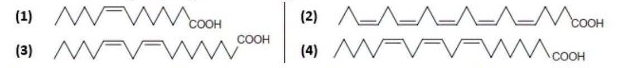
\includegraphics[width=13.5cm]{images_bacninh_12_ma013/cau6_acid_beo.png}
\end{center}
\choice
{3}
{\True 4}
{2}
{1}
\end{ex}
\begin{ex}
Thủy phân hoàn toàn hỗn hợp phenyl acetate và ethyl acetate trong dung dịch $\ce{NaOH}$, thu được sản phẩm gồm
\choice
{\True 2 muối và 1 alcohol}
{2 muối và 2 alcohol}
{1 muối và 1 alcohol}
{1 muối và 2 alcohol}
\end{ex}
\begin{ex}
Ester X có công thức phân tử là $\ce{C4H8O2}$, X có khả năng tham gia phản ứng với dung dịch $\ce{AgNO3}$ trong $\ce{NH3}$. Số công thức cấu tạo của ester X thỏa mãn điều kiện trên là
\choice
{3}
{4}
{\True 2}
{1}
\end{ex}
\begin{ex}
Các khí sinh ra trong thí nghiệm phản ứng của saccharose với dung dịch $\ce{H2SO4}$ đặc bao gồm
\choice
{$\ce{SO2}$, $\ce{H2S}$}
{\True $\ce{CO2}$, $\ce{SO2}$}
{$\ce{CO2}$, $\ce{SO3}$}
{$\ce{CO2}$, $\ce{H2S}$}
\end{ex}
\begin{ex}
Để tráng một lớp bạc lên ruột phích, người ta cho chất X phản ứng với lượng dư dung dịch $\ce{AgNO3}$ trong $\ce{NH3}$, đun nóng nhẹ 60--70$^\circ\text{C}$. Chất X là
\choice
{tinh bột}
{ethyl acetate}
{saccharose}
{\True glucose}
\end{ex}
\begin{ex}
Trong quá trình trồng trọt, người nông dân được khuyến cáo không bón vôi sống (thành phần chính là $\ce{CaO}$) cùng với phân đạm ammonium. Nguyên nhân của khuyến cáo này là
\choice
{\True thất thoát đạm vì giải phóng ammonia}
{tạo thành hỗn hợp gây cháy nổ}
{tạo acid làm ảnh hưởng tới cây trồng}
{làm tăng độ chua của đất}
\end{ex}
\begin{ex}
Công thức phân tử nào sau đây không thể của ester?
\choice
{$\ce{C3H6O2}$}
{\True $\ce{C3H8O2}$}
{$\ce{C3H4O2}$}
{$\ce{C4H6O2}$}
\end{ex}
\begin{ex}
Polysaccharide X là chất rắn, màu trắng, dạng sợi, trong bông nõn có gần 98\% chất X. Chất X là
\choice
{glucose}
{\True cellulose}
{maltose}
{saccharose}
\end{ex}
\begin{ex}
Có nhiều vụ tai nạn giao thông xảy ra do người lái xe uống rượu. Hàm lượng alcohol ethanol trong máu người lái xe không được vượt quá 0,02\% theo khối lượng. Để xác định hàm lượng đó ta chuẩn độ alcohol bằng $\ce{K2Cr2O7}$ trong môi trường acid theo phản ứng:\\
$3\ce{CH3CH2OH} + \ce{K2Cr2O7} + 4\ce{H2SO4} \rightarrow 3\ce{CH3CHO} + \ce{Cr2(SO4)3} + \ce{K2SO4} + 7\ce{H2O}$\\
Khi chuẩn độ 25,0 gam huyết tương máu của một người lái xe cần dùng 20,0 mL dung dịch $\ce{K2Cr2O7}$ 0,010M. Nồng độ phần trăm ethanol trong 25 gam huyết tương máu của một người lái xe là
\choice
{\True 0,11\%}
{0,03\%}
{0,05\%}
{0,027\%}
\end{ex}
\begin{ex}
Cho phản ứng hóa học sau: $\ce{CH3COOH(l) + CH3OH(l) <=> CH3COOCH3(l) + H2O(l)}$. Biểu thức tính hằng số cân bằng nồng độ $K_{\text{C}}$ của phản ứng trên là
\choice
{\True $K_{\text{C}} = \dfrac{[\ce{CH3COOCH3}][\ce{H2O}]}{[\ce{CH3COOH}][\ce{CH3OH}]}$}
{$K_{\text{C}} = \dfrac{[\ce{CH3COOCH3}]}{[\ce{CH3COOH}][\ce{CH3OH}]}$}
{$K_{\text{C}} = \dfrac{[\ce{CH3COOH}][\ce{CH3OH}]}{[\ce{CH3COOCH3}][\ce{H2O}]}$}
{$K_{\text{C}} = \dfrac{[\ce{CH3COOH}][\ce{CH3OH}]}{[\ce{CH3COOCH3}]}$}
\end{ex}
\begin{ex}
Methyl acrylate là một chất kích thích mạnh, có thể gây chóng mặt, đau đầu, hoa mắt và khó thở khi tiếp xúc với da hoặc hít phải, ester này có công thức cấu tạo thu gọn là
\choice
{$\ce{CH3COOC2H5}$}
{$\ce{CH3COOCH3}$}
{$\ce{C2H5COOCH3}$}
{\True $\ce{CH2=CHCOOCH3}$}
\end{ex}
\begin{ex}
Phương trình hoá học của phản ứng hydrate hóa ethylene để điều chế ethanol là: $\ce{CH2=CH2 + H2O -> CH3CH2OH}$. Giai đoạn (1) trong cơ chế của phản ứng trên xảy ra như sau:
\begin{center}
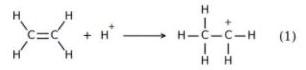
\includegraphics[width=7.5cm]{images_bacninh_12_ma013/cau17_co_che.png}
\end{center}
Nhận định nào sau đây \textbf{không đúng}?
\choice
{Phản ứng hydrate hóa ethylene là phản ứng cộng}
{Trong giai đoạn (1) có sự phân cắt liên kết $\pi$}
{Trong giai đoạn (1) có sự hình thành liên kết $\sigma$}
{\True Trong phân tử ethylene có 6 liên kết $\sigma$}
\end{ex}
\begin{ex}
Tiến hành thí nghiệm theo các bước sau:\\
• Bước 1: Cho khoảng 2mL dung dịch $\ce{AgNO3}$ 1\% vào ống nghiệm sạch.\\
• Bước 2: Thêm từ từ từng giọt dung dịch ammonia 5\%, lắc đều cho đến khi kết tủa tan hết. Dung dịch thu được là thuốc thử Tollens.\\
• Bước 3: Thêm tiếp khoảng 2mL dung dịch glucose 2\% lắc đều. Sau đó, ngâm ống nghiệm vào cốc thuỷ tinh chứa nước nóng trong vài phút.\\
Phát biểu nào sau đây sai?
\choice
{Sản phẩm hữu cơ thu được sau bước 3 là ammonium gluconate}
{\True Thí nghiệm trên chứng minh glucose có tính chất của polyalcohol}
{Sau bước 3, có lớp bạc (silver) kim loại bám trên thành ống nghiệm}
{Trong phản ứng ở bước 3, glucose đóng vai trò là chất khử}
\end{ex}
\vspace{6pt}
\noindent
{\color{mainGreen}\textbf{\large PHẦN II. Câu trắc nghiệm đúng sai}}\\
\textit{\small Thí sinh trả lời từ câu 19 đến câu 22. Trong mỗi ý a), b), c), d) ở mỗi câu, thí sinh chọn đúng hoặc sai.}
\vspace{2pt}

\begin{ex}
Methyl cinnamate là một ester có công thức phân tử $\ce{C10H10O2}$ và có mùi thơm của dâu tây (strawberry) được sử dụng trong ngành công nghiệp hương liệu và nước hoa.
\begin{center}
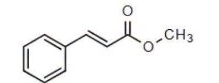
\includegraphics[width=5.5cm]{images_bacninh_12_ma013/cau19_methyl_cinnamate.png}
\end{center}
\choiceTF
{\True Methyl cinnamate có đồng phân hình học.}
{Methyl cinnamate có công thức cấu tạo là $\ce{CH3COO-CH=CH-C6H5}$.}
{Methyl cinnamate phản ứng với $\ce{NaOH}$ với tỉ lệ $1 : 2$.}
{\True Để điều chế 24,3 gam ester methyl cinnamate, người ta cho 29,6 gam cinnamic acid phản ứng với lượng dư methyl alcohol. Hiệu suất phản ứng ester hóa trong trường hợp này là 75\%.}
\end{ex}
\begin{ex}
Tiến hành thí nghiệm điều chế ethyl acetate theo các bước sau đây:\\
• Bước 1: Cho 1mL $\ce{C2H5OH}$, 1mL $\ce{CH3COOH}$ và vài giọt dung dịch $\ce{H2SO4}$ đặc vào ống nghiệm.\\
• Bước 2: Lắc đều ống nghiệm, đun cách thủy (trong nồi nước nóng) khoảng 5 -- 6 phút ở 60 -- 70$^\circ\text{C}$.\\
• Bước 3: Làm lạnh, sau đó rót 2mL dung dịch $\ce{NaCl}$ bão hòa vào ống nghiệm.
\choiceTF
{\True Ở bước 1, có thể thay bằng dung dịch $\ce{H3PO4}$ đậm đặc.}
{Mục đích chính của việc thêm dung dịch $\ce{NaCl}$ bão hòa là để tránh phân hủy sản phẩm.}
{\True Sau bước 3, chất lỏng trong ống nghiệm tách thành hai lớp.}
{\True $\ce{H2SO4}$ đặc có vai trò vừa làm chất xúc tác vừa làm tăng hiệu suất tạo sản phẩm.}
\end{ex}
\begin{ex}
Hợp chất hữu cơ mạch hở X ($\ce{C7H10O5}$) tác dụng với lượng dư dung dịch $\ce{NaOH}$ đun nóng thu được glycerol và hỗn hợp 2 muối carboxylate Y và Z ($M_{\text{Y}} < M_{\text{Z}}$).
\choiceTF
{\True Y tham gia phản ứng tráng bạc.}
{Có 2 công thức cấu tạo thỏa mãn tính chất của X.}
{\True X là hợp chất hữu cơ tạp chức.}
{Carboxylic acid của muối Z có đồng phân hình học.}
\end{ex}
\begin{ex}
Thực vật sử dụng quá trình quang hợp để chuyển đổi năng lượng ánh sáng từ mặt trời thành năng lượng hóa học. Trong quá trình quang hợp xảy ra phản ứng giữa khí carbonic và nước theo phương trình hóa học:\\
$6\ce{CO2(g) + 6H2O(l) -> C6H12O6(aq) + 6O2(g)}$\\
Cho enthalpy tạo thành chuẩn của $\ce{CO2(g)} = -393{,}5\text{ kJ/mol}$; $\ce{H2O(l)} = -285{,}8\text{ kJ/mol}$; $\ce{C6H12O6(aq)} = -1271\text{ kJ/mol}$.
\choiceTF
{Phản ứng quang hợp của cây xanh là phản ứng tỏa nhiệt.}
{\True Nhiệt tạo thành chuẩn của $\ce{O2(g)}$ bằng 0.}
{Biến thiên enthalpy chuẩn của phản ứng trên có giá trị là $-2804{,}8\text{ kJ}$.}
{\True Trồng nhiều cây xanh sẽ làm giảm được nhiệt độ của môi trường xung quanh.}
\end{ex}
\vspace{6pt}
\noindent
{\color{mainGreen}\textbf{\large PHẦN III. Câu trắc nghiệm trả lời ngắn}}\\
\textit{\small Thí sinh trả lời từ câu 23 đến câu 28.}
\vspace{2pt}

\begin{ex}
Có các phát biểu sau:\\
(1) Thủy phân chất béo trong môi trường kiềm luôn thu được glycerol.\\
(2) Triolein làm mất màu nước bromine.\\
(3) Các ester chỉ được điều chế từ carboxylic acid và alcohol.\\
(4) Benzyl acetate là ester có mùi chuối chín.\\
(5) Đốt cháy ethyl acetate thu được số mol nước bằng số mol khí carbonic.\\
(6) Hydrogen hoá hoàn toàn chất béo lỏng (xúc tác Ni, $t^\circ$) thu được chất béo rắn.\\
Liệt kê theo trình tự từ nhỏ đến lớn các số ứng với các phát biểu đúng trên (ví dụ: 56, 124, 3456,...).

\textit{Trả lời:} \dotfill
\end{ex}
\begin{ex}
Cho các phản ứng được đánh số thứ tự như sau:\\
(1) $6n\ce{CO2} + 5n\ce{H2O} \xrightarrow{\text{ánh sáng}} (\ce{C6H10O5})_n + 6n\ce{O2}$\\
(2) $(\ce{C6H10O5})_n + n\ce{H2O} \xrightarrow{\text{enzyme}} n\ce{C6H12O6}$\\
(3) $\ce{C6H12O6} \xrightarrow{\text{enzyme}} 2\ce{C2H5OH} + 2\ce{CO2}$\\
(4) $\ce{C2H5OH} + 3\ce{O2} \rightarrow 2\ce{CO2} + 3\ce{H2O}$\\
Gán số thứ tự phương trình hoá học của các phản ứng theo tên gọi: lên men rượu, thủy phân, cháy, quang hợp và sắp xếp theo trình tự thành dãy bốn số.

\textit{Trả lời:} \dotfill
\end{ex}
\begin{ex}
Một nhà máy đường trung bình mỗi ngày sử dụng 3000 tấn mía để sản xuất. Sau khi nước mía được cô đặc và kết tinh để lấy đường cát, phần chất lỏng màu nâu sẫm, đặc sệt còn lại chính là rỉ đường. Tỷ lệ rỉ đường bằng 4\% khối lượng mía ban đầu. Thành phần chính của rỉ đường gồm: Saccharose (khoảng 40\%), monosaccharide (tổng glucose và fructose khoảng 15\%), nước và các khoáng chất. Nhằm tận dụng nguồn nguyên liệu, nhà máy dùng rỉ đường để sản xuất ethanol, người ta pha loãng rỉ đường và tiến hành lên men bằng nấm men (Saccharomyces cerevisiae). Quá trình gồm thuỷ phân saccharose và lên men monosaccharide (cả glucose và fructose đều lên men tạo ethanol). Hiệu suất thuỷ phân Saccharose và lên men đều đạt 90\%, các thành phần khác không tham gia quá trình tạo ethanol. Thể tích dung dịch ethanol 88$^\circ$ trung bình nhà máy sản xuất được trong 1 ngày là $V$ ($\text{m}^3$), biết khối lượng riêng của ethanol nguyên chất là 0,79 g/mL. Giá trị của $V$ bằng bao nhiêu? (Không làm tròn các phép tính trung gian, chỉ làm tròn kết quả cuối cùng đến hàng đơn vị).

\textit{Trả lời:} \dotfill
\end{ex}
\begin{ex}
Xác định giá trị số sóng $\nu$ ($\text{cm}^{-1}$) hấp thụ đặc trưng của nhóm $\ce{C=O}$ (ketone) trên phổ hồng ngoại IR của methyl phenyl ketone cho dưới đây:
\begin{center}
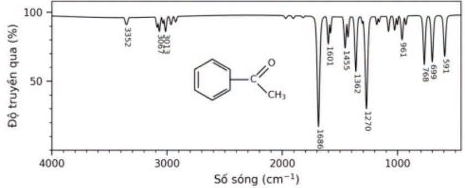
\includegraphics[width=10.5cm]{images_bacninh_12_ma013/cau26_pho_ir.png}
\end{center}

\textit{Trả lời:} \dotfill
\end{ex}
\begin{ex}
Chỉ số xà phòng hoá của chất béo là số mg KOH cần dùng để xà phòng hoá hoàn toàn 1 gam chất béo (bao gồm cả trung hoà acid béo tự do có trong chất béo). Cho bảng số liệu:
\begin{center}
\renewcommand{\arraystretch}{1.15}
\begin{tabular}{|c|c|c|c|}
\hline
\rowcolor{tableGreen}
\textbf{Chất béo} & \textbf{Chỉ số xà phòng hoá} & \textbf{Chất béo} & \textbf{Chỉ số xà phòng hoá} \\
\hline
Dầu dừa & 257 & Dầu olive & 188 \\
\hline
\textbf{Dầu cọ} & \textbf{199} & Mỡ vịt & 194 \\
\hline
Dầu lạc & 192 & Mỡ gà & 195 \\
\hline
Dầu mè & 188 & Mỡ lợn & 198 \\
\hline
\end{tabular}
\end{center}
Giả sử quá trình thực hành điều chế xà phòng, học sinh được yêu cầu điều chế xà phòng từ 200 gam dầu cọ và $\ce{NaOH}$ (rắn). Biết xà phòng được điều chế bằng cách cho chất béo tác dụng vừa đủ với dung dịch $\ce{NaOH}$. Cần cân $m$ (gam) hoá chất từ lọ đựng $\ce{NaOH}$ rắn trong phòng thí nghiệm, biết rằng loại $\ce{NaOH}$ được dùng trong phòng thí nghiệm đã hút ẩm nên lượng $\ce{NaOH}$ chiếm 95\%. Giá trị của $m$ bằng bao nhiêu? (Các quá trình tính toán không làm tròn, kết quả cuối cùng làm tròn đến hàng phần mười).

\textit{Trả lời:} \dotfill
\end{ex}
\begin{ex}
Cho các chất: $\ce{CH3[CH2]14COONa}$, $\ce{CH3[CH2]10CH2OSO3Na}$, $\ce{CH3[CH2]16COOK}$, $\ce{CH3[CH2]7CH=CH[CH2]7COONa}$, $\ce{CH3COONa}$, $(\ce{C15H31COO})_3\ce{C3H5}$. Có bao nhiêu chất có thể là thành phần chính của xà phòng?

\textit{Trả lời:} \dotfill
\end{ex}
\vspace{10pt}
\begin{center}
\textbf{------------------- HẾT -------------------}\\
\textit{\small (Học sinh không được sử dụng tài liệu. Cán bộ coi thi không giải thích gì thêm)}
\end{center}

\end{document}
